\chapter{相关技术与知识}


\section{经典EIM系统总体介绍}

EIM系统的英文全称是 Enterprise Information Management System.  在这个应用中需要首先实现一个适合幼儿园的学生教师人员管理的信息系统, 作为整个系统的数据基础。




一个EPM系统一般使用关系型数据库, 提供Web接口, 让不同用户登录, 同时操作。 并且还需要有一定程度上的权限管理机制。  在当下市场中, 有很多现成的商业化EPM系统, 为公司提供General的解决方案。 


\begin{figure}[H]
	\centering
	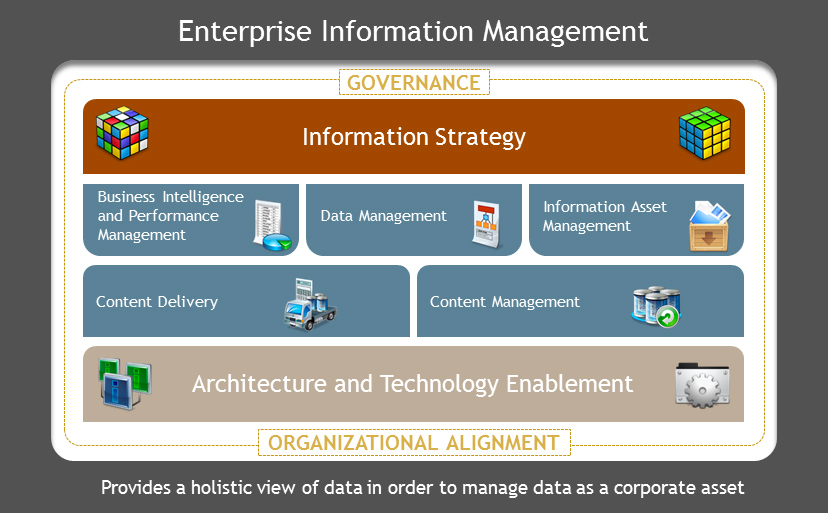
\includegraphics[width=0.80\textwidth]{eim.png}
	\figcaption{Enterprise Information Management System}
	\label{fig: Enterprise Information Management System}
\end{figure}


但这些系统的问题往往是

\begin{itemize}
\item 不领域相关, 而幼儿园有十分独特的人员管理需求
\item 提供了大量不必要的功能
\item 因为功能太多, 也造成使用昂贵
\item 不能加以扩展, 比如支持社交
\end{itemize}

\section{社交SNS类型软件总体介绍}



社交SNS软件是互联网浪潮的一大标志, 它满足了人们的聊天,分享,交友的需求。在这个应用中, 基于管理端的数据, 在老师和家长中做班级为单位的的社交, 所以要实现一个适合该应用场景的社交App.




一般一个社交SNS软件的扩展性, 速度, 及时性十分重要, 而原子性并不强求。 所以大多使用非关系型数据库, 往往都会提供手机App, 不一定提供Web PC应用。在当下市场中, 有很多社交软件, General的社交软件最出名的是 Facebook


\begin{figure}[H]
	\centering
	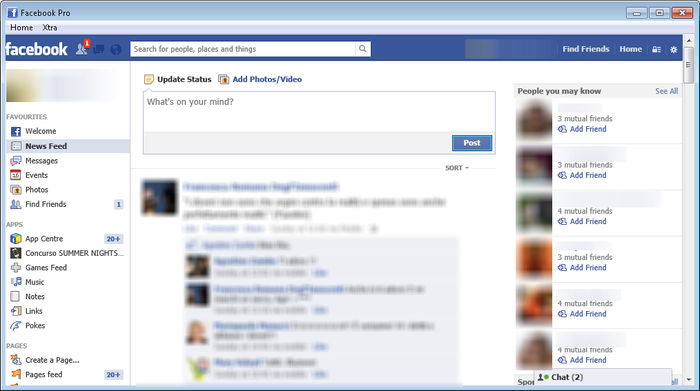
\includegraphics[width=0.80\textwidth]{fb.png}
	\figcaption{facebook}
	\label{fig: fb}
\end{figure}


而对于细分的市场, 各种软件百花齐放。


微信,基于熟人社交

\begin{figure}[H]
	\centering
	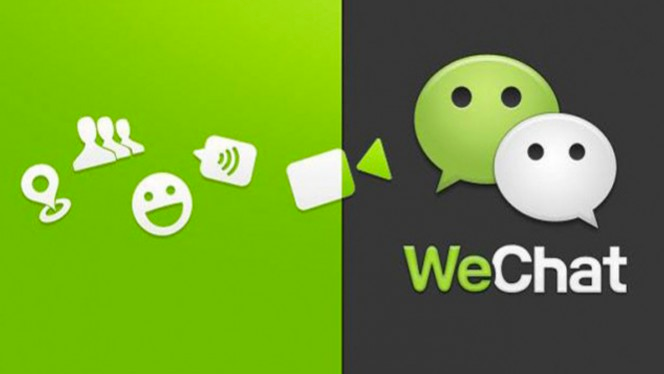
\includegraphics[width=0.80\textwidth]{wechat.png}
	\figcaption{微信}
	\label{fig: wechat}
\end{figure}

陌陌,基于陌生人社交


\begin{figure}[H]
	\centering
	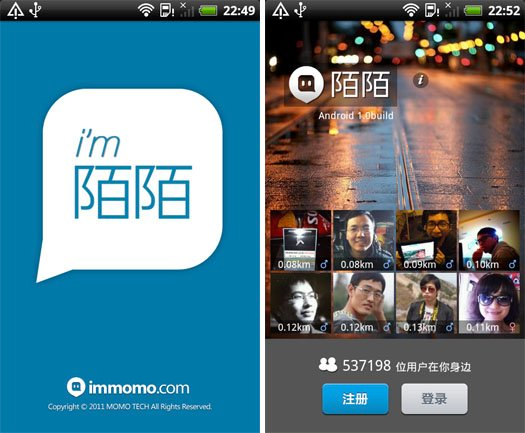
\includegraphics[width=0.80\textwidth]{momo.png}
	\figcaption{陌陌}
	\label{fig: momo}
\end{figure}

Airbnb, 基于租房社交

\begin{figure}[H]
	\centering
	
\includegraphics[width=0.80\textwidth]{airbnb.png}
	\figcaption{airbnb}
	\label{fig: airbnb}
\end{figure}


Spotify, 音乐社交, 基于Facebook

\begin{figure}[H]
	\centering
	
\includegraphics[width=0.80\textwidth]{spotify.png}
	\figcaption{Spotify}
	\label{fig: spotify}
\end{figure}


在这里, 要实现的社交是基于细分的幼儿教育市场。


\section{基于EPM管理系统的社交软件相关技术简介}

对于该应用, 由于要加入社交元素, 加之人员管理系统只需要针对幼教领域来设计功能, 所以使用了非关系型数据库mongodb。 


在Web后端使用了Nodejs来进行程序开发, web前端操作逻辑比较复杂, 所以使用了angularjs前端框架。因为前后端交互比较频繁, 大量使用了websocket而不是Http Ajax访问来进行前后端交互。



App的开发往往比较费时, 尤其是考虑到如何跨平台。 在这里我选用了 Hybrid Html5 Mobile开发框架, 可以使用Web技术来开发 ios \& android 平台app, 一份代码, 两个平台使用。而且Web技术也降低了开发门槛和学习曲线。


\subsection{Nosql 简介}


\begin{figure}[H]
	\centering
	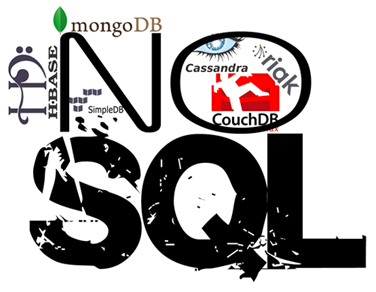
\includegraphics[width=0.80\textwidth]{nosql.png}
	\figcaption{Nosql}
	\label{fig: nosql}
\end{figure}

NoSQL有时也称作Not Only SQL的缩写,是对不同于传统的关联式数据库的数据库管理系统的统称。(注依据Martin Fowler,NoSQL 不是英文Not Only SQL, 因为这会是NOSQL 而不是NoSQL)



两者存在许多显著的不同点,其中最重要的是NoSQL不使用SQL作为查询语言。其数据存储可以不需要固定的表格模式,也经常会避免使用SQL的JOIN操作,一般有水平可扩展性的特征。NoSQL的实现具有二个特征:使用硬盘,或者把随机存储器作存储载体。



当代典型的关联式数据库在一些数据敏感的应用中表现了糟糕的性能,例如为巨量文档建立索引、高流量网站的网页服务,以及发送流式媒体关系型数据库的典型实现主要被调整用于执行规模小而读写频繁,或者大批量极少写访问的事务。



NoSQL的结构通常提供弱一致性的保证,如最终一致性,或交易仅限于单个的数据项。不过,有些系统,提供完整的ACID保证在某些情况​​下,增加了补充中间件层(例如,CloudTPS。有两个成熟的系统有提供快照隔离的列存储:像是Google基于过滤器系统的BigTable,和滑铁卢大学发展的HBase。这些系统,自主开发,使用类似的概念来实现多行(multi-row)分散式ACID交易的快照隔离(snapshot isolation)保证为基础列储存,无需额外的资料管理开销,中间件系统部署或维护,减少了中间件层。



少数NoSQL系统部署了分布式结构,通常使用分散式杂凑表(DHT)将数据以冗余方式保存在多台服务器上。依此,扩充系统时候添加服务器更容易,并且扩大了对服务器失效的承受能程度


\subsection{Mongodb 简介}

\begin{figure}[H]
	\centering
	
\includegraphics[width=0.80\textwidth]{mongo.png}
	\figcaption{mongodb}
	\label{fig: mongo}
\end{figure}


	是由C++语言编写的开源数据库系统。 在高负载的情况下,添加更多的节点,可以保证服务器性能。MongoDB 旨在为WEB应用提供可扩展的高性能数据存储解决方案。
	
	
	
	MongoDB是一种强大、灵活、追求性能、易扩展的数据存储方式。是面向文档的数据库,不是关系型数据库,是NoSQL(not only SQL)的一种。所谓的面向文档,就是将原来关系型数据库中的“行”的概念换成了更加灵活的”文档",以文档为存储单位。文档的值可以是数组、文档等复杂的数据模型。并且文档的键不会事先定义也不会固定不变。mongoDB设计的主要思想之一就是,将能交给客户端的操作都要从服务端转移到客户端,例如生成objectid等操作。
	
	

\subsection{Nodejs 简介}

\begin{figure}[H]
	\centering
	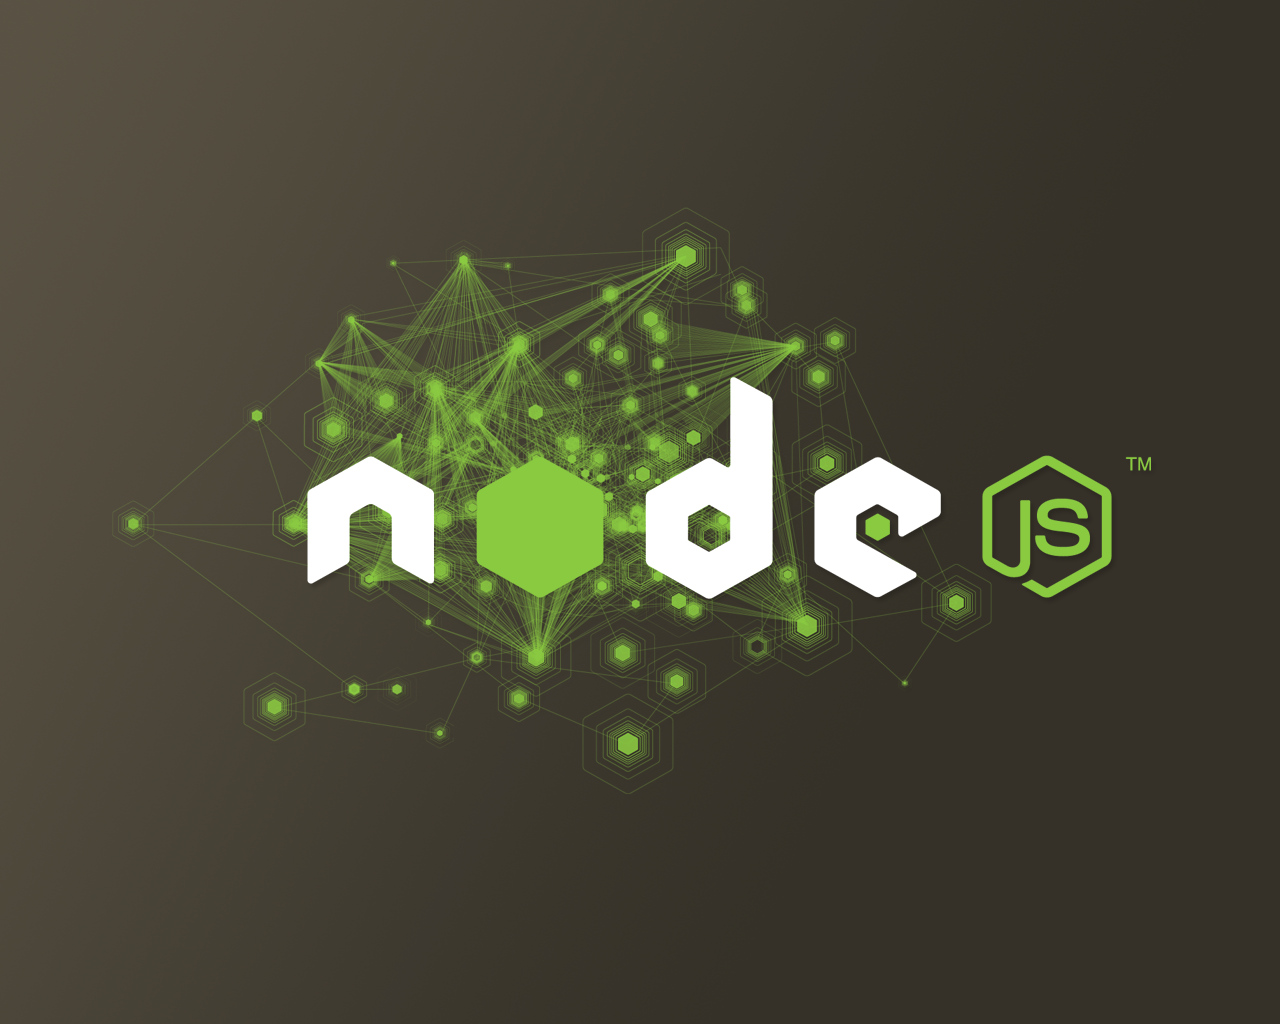
\includegraphics[width=0.80\textwidth]{node.png}
	\figcaption{Node}
	\label{fig: node}
\end{figure}


Node.js是一个基于Chrome JavaScript运行时建立的平台, 用于方便地搭建响应速度快、易于扩展的网络应用。Node.js 使用事件驱动, 非阻塞I/O 模型而得以轻量和高效,非常适合在分布式设备上运行的数据密集型的实时应用。


V8引擎执行Javascript的速度非常快,性能非常好。

Node是一个Javascript运行环境(runtime)。实际上它是对Google V8引擎进行了封装。V8引 擎执行Javascript的速度非常快,性能非常好。Node对一些特殊用例进行了优化,提供了替代的API,使得V8在非浏览器环境下运行得更好。

\subsection{Angularjs 简介}

\begin{figure}[H]
	\centering
	
\includegraphics[width=0.80\textwidth]{ng.png}
	\figcaption{angular}
	\label{fig: angular}
\end{figure}

AngularJS是一款开源JavaScript函式库,由Google维护,用来协助单一页面应用程序运行的。它的目标是透过MVC模式(MVC)功能增强基于浏览器的应用,使开发和测试变得更加容易。

函式库读取包含附加自定义(标签属性)的HTML,遵从这些自定义属性中的指令,并将页面中的输入或输出与由JavaScript变量表示的模型绑定起来。这些JavaScript变量的值可以手工设置,或者从静态或动态JSON资源中获取。

\subsection{Hybrid HTML5 Mobile App 简介}

\begin{figure}[H]
	\centering
	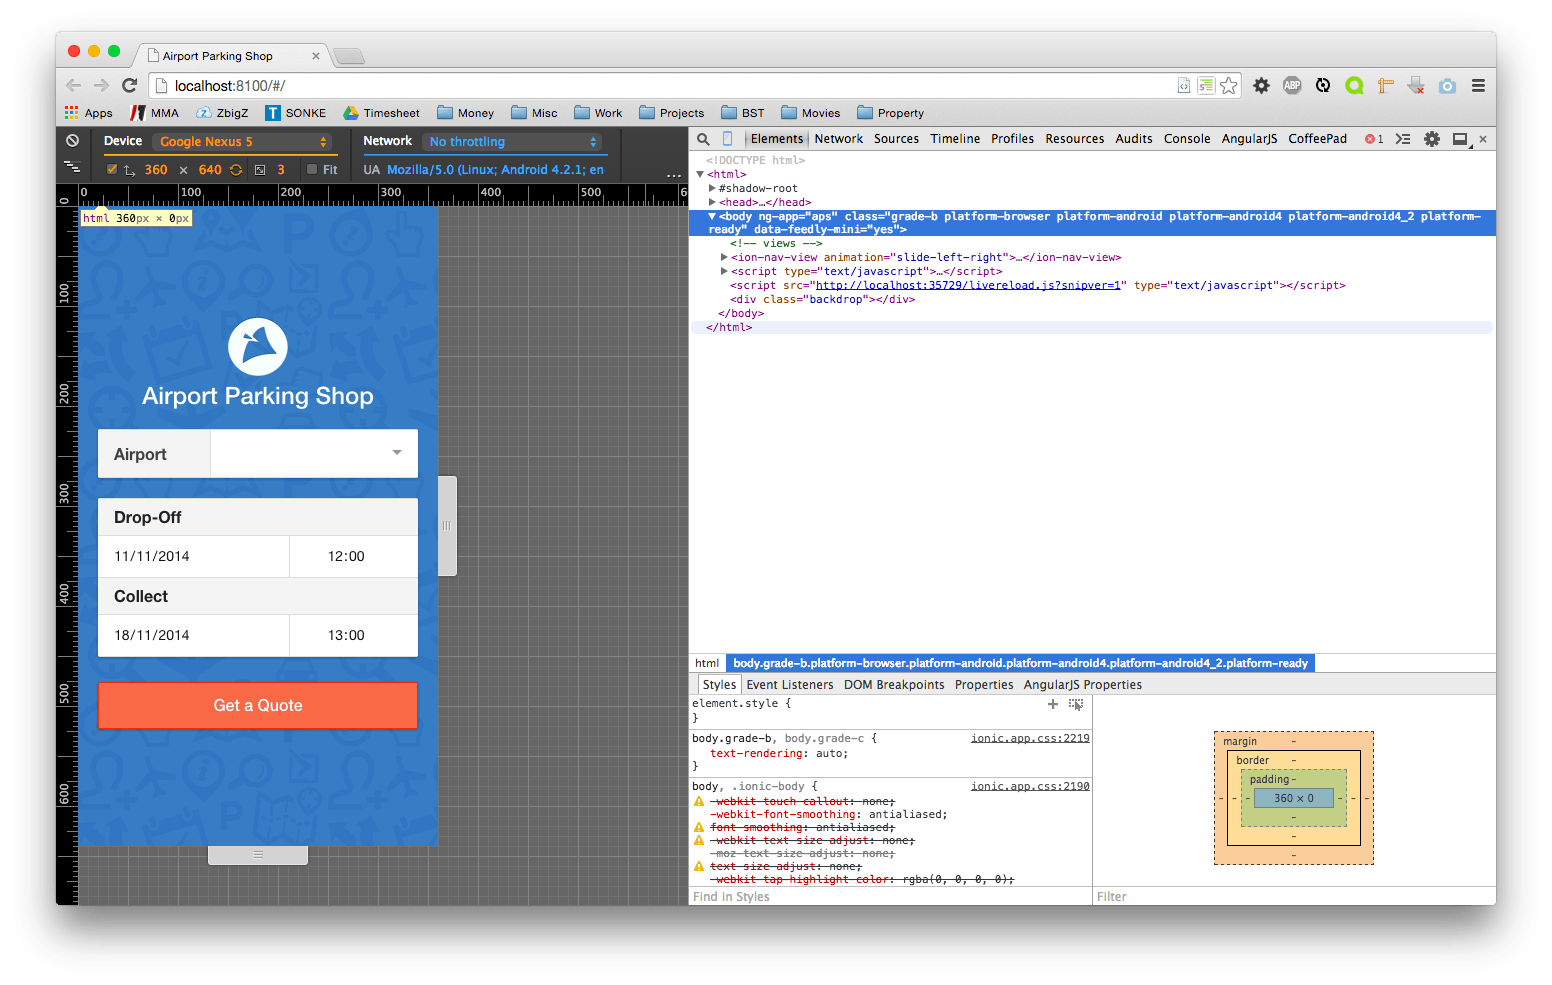
\includegraphics[width=0.80\textwidth]{ionic.png}
	\figcaption{Hybrid App Dev}
	\label{fig: had}
\end{figure}



Hybrid App是指介于web-app、native-app这两者之间的app,它虽然看上去是一个Native App,但只有一个UI WebView,里面访问的是一个Web App,但其通过JSB (javascript Binding)来和系统底层的api交流, 来达到native app的功能, 但却可以使用Web 技术来渲染UI。

另一种方式是使用虚拟的HTML DOM, 把Html Dom来翻译为系统的UI布局代码, 来达到原生应用的UI渲染效率。

现有有很多Html5混合手机开发框架, React Native, ionic等等, 我选用了ionic.


\subsection{WebSocket 简介}

\begin{figure}[H]
	\centering
	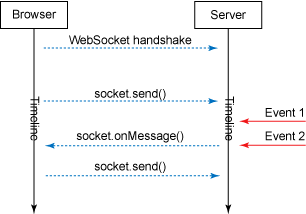
\includegraphics[width=0.80\textwidth]{websocket.png}
	\figcaption{websocket}
	\label{fig: websocket}
\end{figure}

WebSocket是HTML5开始提供的一种在单个 TCP 连接上进行全双工通讯的协议。WebSocket通信协议于2011年被IETF定为标准RFC 6455,WebSocketAPI被W3C定为标准。

在WebSocket API中,浏览器和服务器只需要做一个握手的动作,然后,浏览器和服务器之间就形成了一条快速通道。两者之间就直接可以数据互相传送。